%%%%%%%%%%%%%%%%%%%%%%%%%%%%%%%%%%%%%%%%%%%%%%%%%%%%%%%%%%%%%%%%%%%%%%%%%%%%%
%%%
%%% File: utthesis2.doc, version 2.0jab, February 2002
%%%
%%% Based on: utthesis.doc, version 2.0, January 1995
%%% =============================================
%%% Copyright (c) 1995 by Dinesh Das.  All rights reserved.
%%% This file is free and can be modified or distributed as long as
%%% you meet the following conditions:
%%%
%%% (1) This copyright notice is kept intact on all modified copies.
%%% (2) If you modify this file, you MUST NOT use the original file name.
%%%
%%% This file contains a template that can be used with the package
%%% utthesis.sty and LaTeX2e to produce a thesis that meets the requirements
%%% of the Graduate School of The University of Texas at Austin.
%%%
%%% All of the commands defined by utthesis.sty have default values (see
%%% the file utthesis.sty for these values).  Thus, theoretically, you
%%% don't need to define values for any of them; you can run this file
%%% through LaTeX2e and produce an acceptable thesis, without any text.
%%% However, you probably want to set at least some of the macros (like
%%% \thesisauthor).  In that case, replace "..." with appropriate values,
%%% and uncomment the line (by removing the leading %'s).
%%%
%%%%%%%%%%%%%%%%%%%%%%%%%%%%%%%%%%%%%%%%%%%%%%%%%%%%%%%%%%%%%%%%%%%%%%%%%%%%%

\documentclass[a4paper, 12pt, oneside]{report}         %% LaTeX2e document.
\usepackage {tcdthesis}              %% Preamble.
\usepackage{graphicx,color}
\usepackage{float}
\usepackage{anysize}
\usepackage{amsmath}

\mastersthesis                     %% Uncomment one of these; if you don't
%\phdthesis                         %% use either, the default is \phdthesis.

\thesisdraft                       %% Uncomment this if you want a draft
                                     %% version; this will print a timestamp
                                     %% on each page of your thesis.

\leftchapter                       %% Uncomment one of these if you want
%\centerchapter                      %% left-justified, centered or
% \rightchapter                      %% right-justified chapter headings.
                                     %% Chapter headings includes the
                                     %% Contents, Acknowledgments, Lists
                                     %% of Tables and Figures and the Vita.
                                     %% The default is \centerchapter.

% \singlespace                       %% Uncomment one of these if you want
% \oneandhalfspace                   %% single-spacing, space-and-a-half
 \doublespace                       %% or double-spacing; the default is
                                     %% \oneandhalfspace, which is the
                                     %% minimum spacing accepted by the
                                     %% Graduate School.

\renewcommand{\thesisauthor}{Stroughair Michael}            %% Your official UT name.
\renewcommand{\thesismonth}{October}                  %% Your month of graduation.
\renewcommand{\thesisyear}{2017}                      %% Your year of graduation.
\renewcommand{\thesistitle} {\LARGE{Quantifying Visibility in Volumetric Rendering with Compute Shaders}}            %% The title of your thesis; use mixed-case.
\renewcommand{\thesisauthorpreviousdegrees}{B.A.I.}  %% Your previous degrees, abbreviated; separate multiple degrees by commas.
\renewcommand{\thesissupervisor}{Dingliana John}      %% Your thesis supervisor; use mixed-case and don't use any titles or degrees.
% \renewcommand{\thesiscosupervisor}{}                %% Your PhD. thesis co-supervisor; if any.

% \renewcommand{\thesiscommitteemembera}{}
% \renewcommand{\thesiscommitteememberb}{}
% \renewcommand{\thesiscommitteememberc}{}
% \renewcommand{\thesiscommitteememberd}{}
% \renewcommand{\thesiscommitteemembere}{}
% \renewcommand{\thesiscommitteememberf}{}
% \renewcommand{\thesiscommitteememberg}{}
% \renewcommand{\thesiscommitteememberh}{}
% \renewcommand{\thesiscommitteememberi}{}

\renewcommand{\thesisauthoraddress}{Dublin, Ireland}

%\renewcommand{\thesisdedication}{...}     %% Your dedication, if you have one; use "\\" for linebreaks.


%%%%%%%%%%%%%%%%%%%%%%%%%%%%%%%%%%%%%%%%%%%%%%%%%%%%%%%%%%%%%%%%%%%%%%%%%%%%%
%%%
%%% The following commands are all optional, but useful if your requirements
%%% are different from the default values in utthesis.sty.  To use them,
%%% simply uncomment (remove the leading %) the line(s).

% \renewcommand{\thesiscommitteesize}{...}
                                     %% Uncomment this only if your thesis
                                     %% committee does NOT have 5 members
                                     %% for \phdthesis or 2 for \mastersthesis.
                                     %% Replace the "..." with the correct
                                     %% number of members.

\renewcommand{\thesisdegree}{Master of Science in Computer Science}  %% Uncomment this only if your thesis
                                     %% degree is NOT "DOCTOR OF PHILOSOPHY"
                                     %% for \phdthesis or "MASTER OF ARTS"
                                     %% for \mastersthesis.  Provide the
                                     %% correct FULL OFFICIAL name of
                                     %% the degree.

\renewcommand{\thesisdegreeabbreviation}{M.Sc.}
                                     %% Use this if you also use the above
                                     %% command; provide the OFFICIAL
                                     %% abbreviation of your thesis degree.

\renewcommand{\thesistype}{Dissertation}    %% Use this ONLY if your thesis type
                                     %% is NOT "Dissertation" for \phdthesis
                                     %% or "Thesis" for \mastersthesis.
                                     %% Provide the OFFICIAL type of the
                                     %% thesis; use mixed-case.

% \renewcommand{\thesistypist}{...}  %% Use this to specify the name of
                                     %% the thesis typist if it is anything
                                     %% other than "the author".

%%%
%%%%%%%%%%%%%%%%%%%%%%%%%%%%%%%%%%%%%%%%%%%%%%%%%%%%%%%%%%%%%%%%%%%%%%%%%%%%%

\graphicspath{{images/}}

\begin{document}                                  %% BEGIN THE DOCUMENT

\thesistitlepage                                  %% Generate the title page.

\thesisdeclarationpage				  %% Generate the declaration page.

\thesispermissionpage				  %% Generate the copyright permission page

%\thesisdedicationpage                             %% Generate the dedication page.

\begin{thesisacknowledgments}                     %% Use this to write your
			                          %% acknowledgments; it can be anything
Give many thanks and stuff...

\end{thesisacknowledgments}                       %% allowed in LaTeX2e par-mode.

\begin{thesisabstract}

In Volumetric Rendering applications, understanding what aspects of the data are visible to the user is an important step in optimizing the expressiveness of the image, leading to a better final render.

The aim of this thesis is to design an algorithmic process by which visibility aspects of a Volumetrically Rendered object can be computed in real time. The two taken into consideration within this thesis are the saliency of the data set, and the relative visibility of the individual data points within the final rendered image.


\end{thesisabstract}

\tableofcontents                                  %% Generate table of contents.
\listoftables                                     %% Uncomment this to generate list of tables.
\listoffigures                                    %% Uncomment this to generate list of figures.

%%
%% Include thesis chapters here...
%%
  \chapter{Overview}

The contents of this thesis fall within the research area known as Direct Volume Rendering, or DVR. In the vast majority of cases, an object is rendered using a polygonal mesh to represent its surface geography, and textured using a static image. The lighting applied to this mesh can be described using a Bidirectional Reflectance Distribution function, or BRDF, a surface rendering algorithm that only solves for light from the surface points of an object. As such, when information from the internal structure of an object is required, this method is not suitable.

Direct Volume Rendering techniques allow for the internal structure of an object to be taken into account when rendering the surface image. In these cases, the information cannot be stored simply within a 2D image, but instead within a volumetric grid. This grid consists of image slices sampled from the original object at regular intervals, with each slice containing a regular pattern of elements. The elements of information contained within this grid are known as voxels, the 3D counterpart to pixels. At lower resolutions of data, volumetrically rendered objects appear to be made up of tiny cubes, each of which is a voxel.

Voxels are assigned what is known as an intensity or a material value. This range for this value can vary depending on the data set, but generally it is set between 0 and 255. Using what is known as a Transfer Function, these material values are mapped to an RGBA colour. In many cases, this transfer function doesn't assign each individual material a colour, but instead assigns a colours to ranges of materials. 

This project deals with the question of visibility within this 3D dataset. With the data stored and rendered in this way, it is possible for important features to be hidden behind less important ones. While the alpha values of particular materials can be changed within the transfer function to better see or ignore it, this is a time consuming process, and automation is preferable. Many algorithms have been developed to deal with this problem with varying degrees of success. 

This thesis aims to calculate information for a volumetric gridset on a per-voxel basis in real time, for the purpose of being used by other researchers to better automate and optimise their visibility algorithms. The two information types dealt with are voxel visibility and saliency. 

The Visibilitity of a voxel is a measure of how influencial that voxel is to the final image. The visibility of materials within a volumetric grid is well established, through the creation of visibility histograms etc, but in many cases, researchers wish to know the visibility of individual voxels within the final rendered image. For this reason, visibility fields were introduced, which contain the visibility of each individual voxel within the grid. Saliency is a measure of how noticible a voxel is based on the colour assigned to it by the transfer function. To compute this, the idea of a saliency field was introduced. Unlike a visibility field, a saliency field is view independent, and so does not need to be recalculated each time the camera moves relative to the object.

Calculating these fields can be quite expensive, and while it is possible to do these calculations through the rendering pipeline, it is not made for this purpose. However, OpenGL introduced a new type of shader known as a Compute Shader. Compute Shaders are general purpose shaders, built for large calculations. This makes them perfect for the calculations required by this project. Unlike other solutions available such as CUDA and OpenCL, Compute Shaders are native to OpenGL and so do not require any external files to run. They also are coded through GLSL, making them ideal for new users with experience in shader design.

\section{Structure}

The structure of this thesis is as follows: Chapters 2 and 3 provide an overview of related work within the fields that this thesis is a part of. Chapter 2 talks about Volumetric Rendering, briefly talking about the history before moving into the main techniques used. Chapter 3 provides an explanation of Compute Shaders. Chapter 4 details the implementation of the project, and how each of the core components operate. Chapter 5 walks through the evaluation of the project, presenting the results that were obtained during testing. Chapter 6 is a summary of the work. 
                                
  \chapter{Volumetric Rendering}

This chapter discusses Volumetric Rendering. 

\section{Volume Data}

Here, I want to make clear what exactly is being rendered in a volumetric rendering pipeline, and what makes it different to conventional rendering.

\section{Direct Volume Rendering}

Here, I want to give a quick overview of what is happening. Basically, I want to talk about how its mapping the intensity values contained within the dataset to colours and alpha values from the transfer function onto the image plane

\subsection{Direct Volume Rendering Methods}

Here, I'll go into how its all supposed to work at a low level, give a good amount of detail. I'll first talk about object order approaches, since I'll need to have readers well versed in the idea for when I describe my Compute Shader implementation. Then I'll chat about image order approaches, to help understand the raytracing aspect of the program.
\subsubsection{Object-Order Approaches}

Here's some words

\subsubsection{Image-Order Approaches}

Here's some more words

\section{Visualisation}

                                
  \chapter{Compute Shaders}

Will this chapter even need sections? Honestly, I don't know. 

\section{A section of more Stuff}

Blah, blah, blah! Blah, blah, blah! Blah, blah, blah!

Blah, blah, blah! Blah, blah, blah! Blah, blah, blah!



  \chapter{Implementation}

This chapter explains the implementation of the project goals. A Volumetric Renderer was provided initially to allow for more time to be devoted to the project's implementation rather than for its creation. Many portions of this original code still remain, however much of it was refactored or replaced during the project, to allow for better readability and useability.

The chapter is divided into two main sections. The first section deals with the shaders created during the project period. The second section breaks down the code that runs on the CPU. 

\section{Shader Design}

This section contains two subsections. The first looks at the work done by the Compute Shader in calculating the Visibility Field. The second looks at the work done in calculating the saliency field.

\subsection{Volumetric Rendering Shader}

This shader was provided as part of the Renderer supplied at the start of the project period. It implements a ray marching algorithm for calculating the colour for each fragment from the data volume provided.

The code works by first finding the normalised direction vector from the camera to the current fragment. The absorption for that fragment is set to $0.0$, and the code enters the main loop. Within this loop, the colour for that position within the data volume is calculated, multiplied by its opacity value, and added to the total colour (set to $(0.0, 0.0, 0.0, 0.0)$ initially). The opacity of the colour is added to the absorption for the fragment. The next sampling position is calculated by moving along the direction vector. 

At this point, the algorithm determines whether it needs to continue. If the new position is outside the bounds of the data volume, or if the absorption of the fragment is equal or greater than 1.0, then it can return the current colour value. Otherwise, it calculates the colour for that new position, multiplies it again by the opacity value, and adds it to the total colour.

A later addition to this code was the ability to draw a border along the edge of the volume, for aesthetic purposes. If the initial position of the fragment is within a tolerance of the edge of the volume, the final colour outputted is black. In each data volume used, there is no relevant information stored this close to the edge of the volume, so it has no effect on viewing the final image. It does however serve to better understand where the camera is with relation to the primary axes.

\subsection{Visibility Field Shader}

When developing this shader, the problem of coordinate space was a constant concern. The data volume and camera are always within world space, which centers the object on (0,0,0), and the camera relative to this. However, the data volume is only accessible via texture space, where (0,0,0) is a corner of the volume. This required a number of conversion functions to be written to accomodate this.

The calculations are performed per voxel, taking full advantage of the design of the compute shader by assigning each voxel to a shader invocation. The algorithm then inspiration from per-voxel volumetric rendering by raymarching from the voxel to the camera, calculating the opacity of the voxel relative to the voxels in front of it. This is achieved by subtracting the opacity of any voxels encountered during the raymarch from the current opacity of the voxel. If this opacity drops below 0, the voxel is not visible at all to the user, and the algorithm ends early. If the algorithm detects that it is outside of the limits of the volume, it also ends early.

The second problem that was encountered was one of sampling frequency. One issue with raymarching algorithms for volumetric rendering is how often should the ray sample the data to get one sample per voxel. Along any of the primary axes this is simply half the length of a voxel, but when projecting along any other line, this distance is different. The solution however to this was quite simple. Previously, the data volume and the output volume were passed to the shader using the $Image3D$ texture format. This allows data to be written to a variable and outputted back to the CPU, an important aspect to my solution. This limits the access of this data to integer values, meaning no interpolation. To negate the need for a variable sampling frequency, all that was required was to change the input of the data volume to a $Sampler3D$ format, and interpolate the opacity value required.

\subsection{Saliency Field Shader}

In most edge detection algorithms, a filter is applied to a greyscale version of the data. This would not be suitable in this case however, due to the importance of colour in depicting saliency. To mitigate this, the intensity of the colour for a voxel is determined by calculating the length of the 3D colour vector, and multiplying it by the opacity value. This is then used with the filter to determine the value of the gradient in an area.

The laplacian filter used here can be quite susceptible to noise, so a variable named $lowerLimit$ was included, whose value is user determined. In the case that the total value for a voxel is less than the value of $lowerLimit$, the voxel's value is set to 0.

\section{CPU Code Design}

This section deals with the code written to run on the CPU. The first section details how the Compute Shader is initialised and run. The second section explains the layout of the final rendered image.

\subsection{Compute Shader Setup}

Compute Shader setup is the same as the setup for Vertex and Fragment Shaders, but it differs in how it is called by the program. Rather than calling $DrawArrays()$, $DispatchCompute()$ is called instead, which requires the size of the local work group to be passed to it. Since the data being computed by the GPU during this time will be required later in the rendering pipeline, it is important to also call $glMemoryBarrier()$ to allow the Compute Shader to finish before continuing so as to ensure that no data hazards occur later on within the code.

\subsection{Display Design}

The code was built with the ability to orbit around each object independently. As such, each object is rendered separately to its own framebuffer object, each with its own camera with movement mapped to different keys. To fit both onto the screen, the horizontal screen size is halved, and each framebuffer is then rendered to a quad. The leftmost quad contains the original data volume, while the rightmost can either contain the visibility field volume or the saliency field volume, depending on the choice of the user.
  \chapter{Evaluation}

This chapter details the tests performed on the Visibility field computation code. The first test shows the difference in computation time between volumes of differing dimensions. The second test compared the computation times for the same volume but with the alpha values within the transfer function changed. The final test altered the size of the local work group within the compute shader to determine the impact on performance.

For each of these tests, the speed was computed as an average over 360 frames, where the volume was rotated 1 degree each time. The measurement was taken using the system clock, and measured only the time it took to setup, call the Compute Shader and then wait for it to return.

\section{Data Used}

The tests detailed below use five different data volumes. These are listed below.

\begin{table}

\begin{center}
\begin{tabular}{l|c}
Data Set & Dimensions (x * y * z) \\
\hline
\hline
Knee & 379 * 229 * 305 \\
Bonsai & 256 * 256 * 256 \\
Engine & 256 * 256 * 110 \\
Tooth & 140 * 120 * 161 \\
Nucleon & 41 * 41 * 41 
\end{tabular}
\end{center}
\caption{\textit{List of data sets used and their size}}
\end{table}

The same transfer function was used for each test, with the exception of  the second test. In this case, new transfer functions were created by reducing the opacities for the original transfer function by a fraction. The transfer function with the lowest opacity values had been assigned values $\frac{1}{4}$ of those from the original, the next with $\frac{1}{2}$, and the final with $\frac{3}{4}$. 

\section{Change in Computation Time against Volume Size}

The aim of this test was to determine whether the computation time of the visibility field changed with a change in the size of the data set, and if so by how much. As shown in the table above, there was a good variety of sizes to test with, and the test resulted in the graph below. As would be expected, the graph suggests a linear relationship between average computation time and the size of the data set. The y-intercept is approximately 15ms, the time it took for the compute shaders to be set up and return the final values.

\begin{figure}[H]
\centering
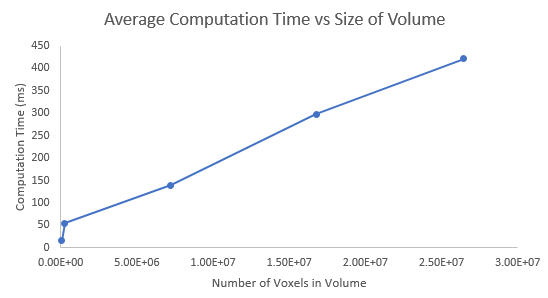
\includegraphics[scale=1.0]{sizes.PNG} 
\caption{\textit{A graph of the average computation times against the size of the data set being worked with}}
\end{figure}

\section{Change in Computation Time against Opacity}

Within the shader code, there is an early exit in the case where the code determines that the voxel is no longer visible behind all the other voxels in front of it. The aim of this test was to determine whether the computation time of the visibility field would change if the opacities of the voxels was changed, and perhaps cause the early exit to be used less often. This was achieved by measuring the speed of the computation against the same transfer function, but each copy of the transfer function having a successively lower opacity value for the most common intensity value over all the data sets. The results are shown below. The data suggests that there could be a small increase with lower opacities for certain intensity values, but the results are inconclusive, given how small the change is.

\begin{figure}[H]
\centering
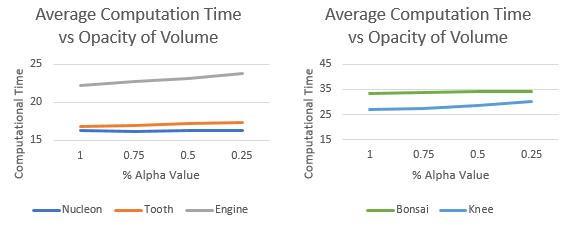
\includegraphics[scale=1.0]{alphaValues} 
\caption{\textit{A graph of the average computation times for each version of the transfer function over a total of 360 frames.}}
\end{figure}

\section{Change in Computation Time against Local Work Group Size}

The impact of the Local Work Group size on the Computation time was an unknown factor within this project. This test was designed to determine whether varying this size had any effect. It was evaluated by measuring the speed of the computation of the visibility field for different sizes of local group. The results are shown in figure 5.1 below. The data points to an exponential decrease in the computation time with an increase in workgroup size in powers of 2.

\begin{figure}[H]
\centering
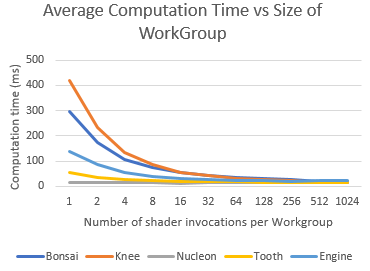
\includegraphics[scale=1.0]{workgroupSize} 
\caption{\textit{A graph of the average computation times for each work group size over a total of 360 frames.}}
\end{figure}

One interesting observation that was made was on the errors that cropped up within the volume during evaluation during this test. While varying the size of each dimension disproportionally had no visible difference from varying each dimension equally, it was noticed that if a single dimension became too large, the resulting volume displayed unusual consequences, such as portions no longer rendering, or refusing to render at all. 

The cause of this error was discovered when the sizes of each volume were determined. The tests were performed for powers of two, but the dimensions of the volumes didn't follow this rule. This caused computational errors to occur as a direct consequence. It is recommended that data volumes undergo a primary step in which the data is transferred into a volume with dimensions of a power of 2, and to also ensure that the work group size is a suitable fraction of the full volume size, so that each work group performs the same amount of work.
  \chapter{Conclusions}

And a fancy conclusion...



%\addcontentsline {toc}{chapter}{Appendices}       %% Force Appendices to appear in contents
\begin{appendix}
\chapter{Abbreviations}

\begin{tabular}{p{40mm}|p{100mm}}
	\textbf{Short Term}&\textbf{Expanded Term}\\
	\hline
	DNS&Domain Name System\\
	DHCP&Dynamic Host Configuration Protocol\\
	...&...
\end{tabular}

%\chapter{Another appendix}

...

\end{appendix}


%\addcontentsline {toc}{chapter}{Bibliography}     %% Force Bibliography to appear in contents

\begin{thebibliography}{ieeetr}                   %% Start your bibliography here; you can
%\bibliography{refs}                               %% also use the \bibliography command

\bibitem{neuro-book-01}
Laurie, Lundy-Ekman. (1998) \underline{Neuroscience: Fundamentals for Rehabilitation.} W.B. Saunders Company, USA.

\bibitem{neuro-book-02}
Purves, D., Augustine, G., Fitzpatrick, D., Hall, W., LaMantia, A., McNamara, J.,Williamos, S. (2004) \underline{Neuroscience:Third Edition} Sinauer Associates, Inc., USA.

\bibitem{neuro-book-03}
Longstaff, A. (2005) \underline{Neuroscience} Second Edition. Taylor and Francis Group, USA.



\end{thebibliography}                             %% to generate your bibliography.


\end{document}                                    %% END THE DOCUMENT
